\section{Model View Controller}\section{sec:mvc}
The Model View Controller (MVC) is a design pattern widely used in programming to separate the program into Model, View, and Controller.
This provides the advantage that the code gains clarity and is easier to maintain as it separates responsibility to individual layers.

An illustration of MVC can be seen in \figref{fig:MVC}.
\begin{figure}[h]
	\centering
	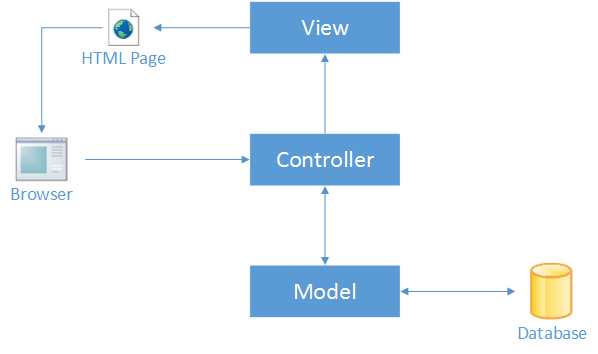
\includegraphics[scale=0.6]{relevantmaterial/MVC}
	\caption{Illustration of MVC pattern.}\label{fig:MVC}
\end{figure}

If you look at the illustration, the `Database' is in our case the relational MySQL database, where data is stored in tables.

The `Model' in our case provides abstraction over the information in the database, it consists of several entities and a service for each such entity.
This is to make the entities simply wrap data, while the services work on the data, and each implement an interface, requiring the services to implement Create, Read, Update, and Delete (CRUD) methods.

The `Controller' provides a set of 'actions' that the user points the browser at. 
These actions then use CRUD methods in the `Model' layer and can also send commands to views to update the view's representation of the model, e.g. a table or a map of stations. 
These views are then presented to the user through the client.
A controller may include multiple views to get a html-page generated for the client to view.
As multiple views may be included by the controller, it may use separate views for the header, the body, and finally one for the footer.

It is important to note that there is a single model layer, consisting of multiple entities (e.g bicycle and booking) and their associated services.
Additionally, it is a good practice to have multiple controllers, which each handle different parts of the website.
In our case we for example have a home and user controller.
With the user controller taking care of everything connected to user login, editing of profile, logout etc.
The home controller takes care of the presentation of the frontpage and the functionality of booking and unbooking of bicycles.
As is evident, the controllers are split into different actions present on the website, which ensures better code clarity.

In addition to the better code clarity, as the website is organised in the way it is, working with the same model, the layout of the website can easily be changed, by including other views or developing additional controllers for other work routines.
This is relates to the high modularity you gain with the MVC pattern, inducing high cohesion and low coupling.